\documentclass[journal, a4paper]{IEEEtran}
\usepackage[utf8]{inputenc} %UTF8 input file
\usepackage[T1]{fontenc}
\usepackage[ngerman]{babel} %Umlaute,Silbentrennung
\usepackage{amssymb} %triangleright
\usepackage{enumitem} %itemize einrücken 
\usepackage{graphicx} %Grafiken einbinden
\usepackage{booktabs} %Tabellen
\usepackage{caption}
\usepackage{amsmath}
\date{\today}
\author{Malte~Ollenschläger}
\title{DIY: Herstellung eines personalisierten Weckers mit Mikrocontroller und mp3-Player}
\begin{document}
\maketitle
\begin{abstract}
	Dieses Dokument beschreibt die Herstellung eines personalisierten Weckers. Das beinhaltet die Erstellung eines Gehäuses und das Schreiben der Software für den Mikrocontroller. Auch die Bauteilauswahl und die Fertigung von Platinen sind in diesem Projekt inbegriffen. Das Ziel ist einerseits die Fertigung des Weckers, andererseits die Durchführung eines Projektes mit verschiedenen Aufgabenbereichen, um das hierbei Gelernte, in folgenden Projekten zu einer effizienteren Arbeitsweise umzusetzen. Dies betrifft sowohl inhaltliche als auch formelle Arbeitsschritte.
\end{abstract}

%\begin{IEEEkeywords}
%mp3-Wecker,
%\end{IEEEkeywords}

\section{Einleitung}
	\IEEEPARstart{D}{ie} Gesamtfunktion des Weckers setzt sich aus mehreren Teilfunktionen zusammen. Eine der grundlegenden Funktionen ist die \textit{Anzeige der Uhrzeit} auf einem Display. Weiterhin wird das \textit{Datum} durch die Zusammensetzung des aktuelle Monats als Wort und des Tages als Ordinalzahl angezeigt. % An ausgewählten Tagen, wie zum Beispiel dem der Besitzerin soll das Display anstatt des Datums eine andere \textit{Zeichenkette oder ein Bild} anzeigen.
	Ein weiteres Symbol gibt an, ob der \textit{Alarm ein- oder ausgeschaltet} ist. Das \textit{Umschalten} funktioniert durch das Gedrückthalten eines Tasters, über den gleichzeitig bei kurzem Drücken die \textit{Displaybeleuchtung} (UND DER FRONTPLATTE) eingeschaltet werden kann. Die Implementierung der \textit{Weckfunktion} sorgt bei eingeschaltetem Alarm dafür, dass zur konfigurierten Uhrzeit der mp3-Player gestartet und eine sich auf selbigem befindliche mp3-Datei abgespielt wird. Beim nächsten Weckruf wird die darauf folgende Datei abgespielt.\par

	Über ein \textit{Menü}, das über das Bedienen eines zweiten Tasters zu erreichen ist, sind folgende Elemente einstellbar:
	\begin{itemize}[leftmargin=20mm]
	\item Uhrzeit
	\item Weckzeit
	\item Datum
	\item Lautstärke
	\item Boombox
%	[$\blacktriangleright$]
	\end{itemize}
	Innerhalb des Menüs findet die Navigation über einen Drehencoder statt.	Bei der Einstellung des Datums wird neben Tag und Monat auch das Jahr abgefragt. Dies dient der \textit{Erkennung von Schaltjahren}, damit in diesen in der Datumsanzeige auf den 28. Februar statt dem 1. März der 29. Februar folgt. Mit dem Menüpunkt "Lautstärke"\ lässt sich eben diese des mp3-Players und damit die \textit{Lautstärke des Wecktons} verändern. Wird der Menüpunkt "Boombox"\ ausgewählt, so kann über ein Cinch-Kabel eine \textit{externe Audio-Quelle} angeschlossen werden und die darauf abgespielte Musik wird über die Lautsprecher des Weckers wiedergegeben. In dieser Zeit ist die Weckfunktion außer Kraft gesetzt.\par
	Die Personalisierung des Weckers wird durch drei Eigenschaften erreicht. Die erste ist die Tatsache, dass die Weckmusik nach dem eigenen Geschmack angepasst werden kann, indem diese auf den mp3-Player kopiert wird. Die zweite personalisierte Eigenschaft ist, dass beispielsweise an Valentinstag und am Geburtstag der Person statt des Datums andere Bilder oder Texte eingeblendet werden. Der offensichtlichste Teil der Personalisierung liegt in der Herstellung des Gehäuses. In die Front des Weckers werden Motive zu denen die Benutzerin einen persönlichen Bezug hat geschnitten. Diese werden zusätzlich zum Display beleuchtet, wenn der entsprechende Taster betätigt wird.
	Als Vorlage für dieses Projekt diente ein ebenfalls selbst hergestellter Wecker, der auf der Internetseite www.wiesolator.de vorgestellt wurde. 
\section{Hardware}
	In diesem Abschnitt wird die genutzte Hardware erläutert. Hierzu wird in Teil \ref{sc:Hardware:subsc:Bauteile} beschrieben, welche Bauteile benötigt werden. Der sich anschließende Teil \ref{sc:Hardware:subsc:Dimensionierung} befasst sich mit der externen Beschaltung der Bauteile. In \ref{sc:Hardware:subsc:Platinen} wird auf die Planung und Fertigung der Platinen eingegangen.
	\subsection{Bauteile}
		\label{sc:Hardware:subsc:Bauteile}
		Der Schaltplan, der im Vorlageprojekt genutzt wurde, dient als Anhaltspunkt für die Hardware, die benötigt wird. Daraus wurde das Schaubild in Abb. \ref{fig:Hierarchie} erstellt, um eine Übersicht der wichtigsten Bauteile zu erhalten.
		\begin{figure}
				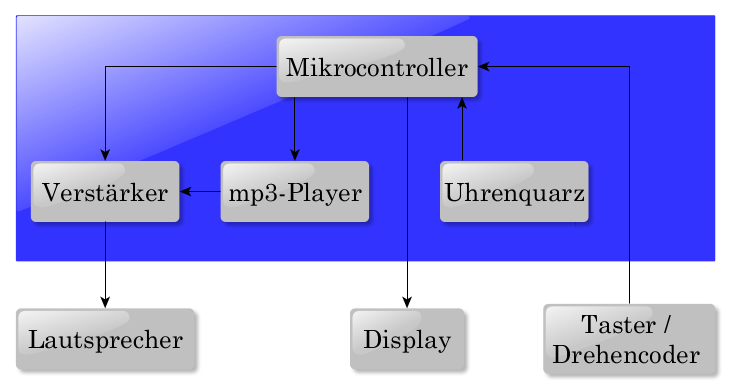
\includegraphics[width=80mm]{./Grafiken/Hierarchie}
				\caption{Hierarchie der Elementaren Bauteile des Weckers. Die Pfeilspitze zeigt in die Datenflussrichtung. Blau unterlegt sind die für den Benutzer nicht zugänglichen Bauteile im Gehäuse. Die unterste Zeile zeigt die Ein- und Ausgabeebene, worüber der Benutzer mit dem Wecker interagiert.}
				\label{fig:Hierarchie}
		\end{figure} 
		Eine Auflistung aller benötigten Bauteile ist in Tabelle \ref{tab:Bauteile} aufgeführt. Die benötigten Widerstände und Kondensatoren sind nicht aufgeführt, da diese den Datenblättern der jeweiligen Bauteile zu entnehmen sind. Zusätzlich werden für das Entprellen der Taster und des Drehencoders 100nF Kondensatoren eingesetzt.
		\begin{center}
			\begin{tabular}{rl}
				\toprule
				Funktionseinheit & Herstellerbezeichnung \\
				\midrule
				Buchsenleiste & EBLG-20-1-X\\
				Display & EA DOGL128W-6 \\
				Displaybeleuchtung & EA LED68x51-W\\
				Drehencoder & STEC11B \\
				Lautsprecher & Visaton FR8-8 \\
				Mikrocontroller & Atmega328P \\
				mp3-Player & Intenso Music Walker \\
				Schaltnetzteil 5V/1A & goobay 54805 \\
				Spannungsregler 1,5VDC & LM317\\
				Spannungsregler 3,3VDC & LM3940 \\
				Spanplatten & \\
				Schrauben &\\
				Muttern&\\
				Taster & FEHLT \\
				Uhrenquarz 32kHz& - \\			
				Verstärker & TDA7266 \\
				\bottomrule		
			\end{tabular}
			\captionof{table}{Benötigte Bauteile. Notwendige Kondensatoren und Widerstände sind nicht angegeben. Diese sind in den jeweiligen Datenblättern zu finden.}
			\label{tab:Bauteile}
		\end{center}
		Neben dieser Hardware werden Spanplatten zur Fertigung des Gehäuses, sowie einige Schrauben benötigt.

	\subsection{Gehäuse}	
		\subsection{Dimensionierung}
			\label{sc:Hardware:subsc:Dimensionierung}
			Grundsätzlich wurden die in den Datenblättern empfohlenen Kondensatoren und Widerstände eingesetzt. Zum Entprellen der Taster sind in den entsprechenden Datenblättern keine Informationen vorhanden. Es werden Keramikkondensatoren der Größe $C=100 nF$ genutzt. Bei dem Spannungsregler für den mp3-Player (LM317) muss eine individuelle Dimensionierung vorgenommen werden, da der Ausgang des gewählten Spannungsreglers variable Spannungen erzeugen kann.
			Die benötigte Versorgungsspannung beträgt $1,5 V$. Nach der im zugehörigen Datenblatt [QUELLE] angegebenen Formel, kann für eine gewünschte Ausgangsspannung die Größe der benötigten Widerstände berechnet werden.  Somit ergibt sich die Größe von $R_2$ nach folgender Gleichung:
			\begin{equation}
				\label{eqn:1,5VDC}
				R_2 = (\frac{V_{out}}{V_{ref}}-1) / (\frac{1}{R_1}+I_{adj})
			\end{equation}	
			Für den Ausgleichsstrom wurden 50$\mu A$ und damit die Hälfte des Maximums angenommen. Dieser wird vom Spannungsregler so geregelt, dass $V_{ref} = 1,25 V$ gilt. Bei einer Wahl von $R_1 = 10k\Omega$ ergibt sich für $R_2 \approx 1,3 k\Omega$.
			Zur Beleuchtung der beiden Bilder auf der Frontseite des Weckers wird eine Transistorschaltung (\ref{fig:Transistor} benötigt. 
			\begin{figure}
				\begin{center}
					\label{fig:Transistor}
					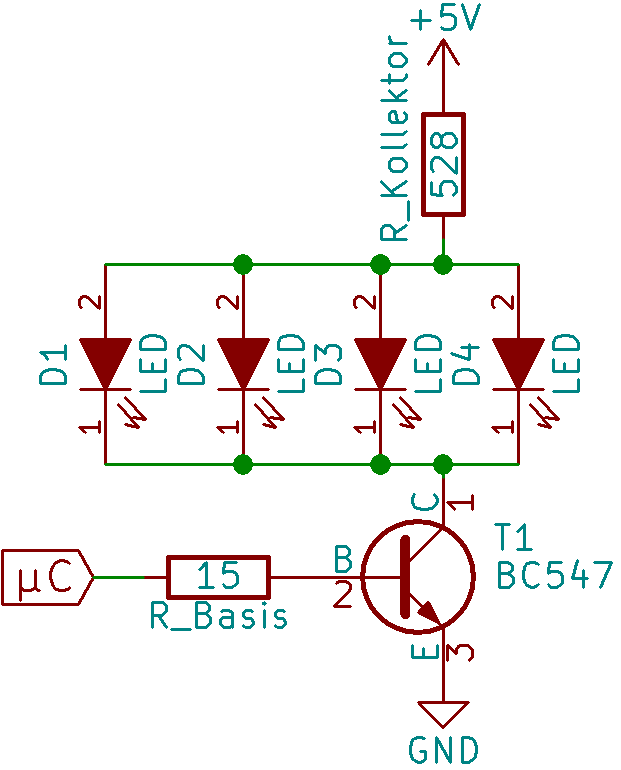
\includegraphics[width=5cm]{./Grafiken/Transistor.png}
					\caption{Transistorschaltung zur Ansteuerung von LEDs}
				\end{center}
			\end{figure}
			Diese wird durch ein Kontrollsignal vom Mikrocontroller, welches an die Basis des Transistors angeschlossen ist, gesteuert. Ein BC547C Transistor schaltet 4 LEDs mit je 20 mA. Die Berechnung der Widerstände ergibt sich aus folgen Formeln: 
			\begin{equation}
				R_{Basis} \leq \frac{U_{\mu C}-U_{BE}}{I_B} =  \frac{3,3V-0,66V}{5mA} \approx 528\Omega
			\end{equation}
			\begin{equation}
				\begin{split}
					R_{Kollektor} = & \frac{U_{cc}-U_{LED}-U_{CE}}{I_{C}} = \\ 
					&\frac{5V-3,6V-0,2V}{80mA} \approx 15\Omega
				\end{split}
			\end{equation}
			Da der Mikrocontroller eine Versorgungsspannung von $3,3V$ hat, ist das Steuersignal $U_\mu C$ ebenso groß. Die Basis-Emitter- und Kollektor-Emitter-Spannung sowie der Basisstrom sind dem Datenblatt des BC547C entnommen. Gleiches gilt für die an den LEDs abfallende Spannung. Nach den Berechnungen in (2) und (3) wurde der Basiswiderstand auf $440\Omega$ und der Kollektorwiderstand auf  $15\Omega$ gewählt.
			Der Kollektorstrom von $I_C=80mA$ ist das Vierfache des Vorwärtsstroms einer LED ($I_F=20mA$), da er sich nach der ersten Kirchhoff'schen Regel gleichmäßig auf die vier LEDs aufteilt.
		\subsection{Gehäuse}
	\subsection{Platinen}
		\label{sc:Hardware:subsc:Platinen}
		Die für dieses Projekt benötigten Platinen wurden mit KiCAD geplant und anschließend im FabLab der Friedrich-Alexander-Universität Erlangen-Nürnberg erstellt. Eine Platine ist für das Display und die zugehörigen Bauelemente (Kondensatoren, Widerstände) ausgelegt. Über einen Steckverbinder kann diese Platine mit einer zweiten verbunden werden, welche die anderen Bauelemente wie zum Beispiel den Mikrocontroller und den Audio-Verstärker enthält. \par
		Für die Displayplatine wurden die Anschlüsse des Displays nicht direkt auf der Platine verlötet. Es wurden Buchsenleisten verlötet in welche das Display samt verlöteter Hintergrundbeleuchtung eingesteckt wird. Dies dient einerseits dazu, dass das Display zum Wechsel oder zur Reparatur ausgebaut werden kann; andererseits dazu, dass der Abstand zwischen Gehäuseinnenseite und Platine vergrößert wird. Dies ist notwendig, damit der Drehencoder, welcher auf der Platine befestigt wird, nicht zu weit nach vorne aus dem Gehäuse herausragt. Außerdem dient es der Herstellung einer kraftschlüssigen Verbindung. In die vier Ecken der Platine werden Löcher gebohrt, ebenso im gleichen Abstandsmaß in die Front des Weckers. Anschließend kann die Platine per Schraube und Mutter von innen gegen das Gehäuse gedrückt werden, sodass das Display fixiert ist und durch die rechteckige Öffnung in der Front des Gehäuses betrachtet werden kann. Für die Erstellung der Platine wurde eine Leiterbahnbreite von $0,5mm$ gewählt, da genug Fläche vorhanden war.\par
		Für die Hauptplatine wurde ebenfalls eine Leiterbahnbreite von $0,5mm$ gewählt. Neben der Displayplatine wurden weitere Bauelemente per Steckverbinder mit der Platine verbunden. Diese sind:
		\begin{itemize}
			\item Lautsprecher
			\item Taster
			\item Drehencoder
			\item LED-Beleuchtung (Bilder)
			\item mp3-Player
		\end{itemize}
	\subsection{Pinbelegung Mikrocontroller}
		\label{sc:Hardware:subsc:Pinbelegung}
		Da es für den Oszillator keine Auswahlmöglichkeiten bezüglich der Pinbelegung gibt, wurden ihm als erstes die entsprechenden Pins zugewiesen. Die Pins für das Displays wurden so gewählt, dass alle nebeneinander liegen, damit das Layout der Platine erleichtert wird und lediglich gerade Leiterbahnen zwischen den Pins des Mikrocontrollers und dem betreffenden Steckverbinder erstellt werden müssen. Gleiches gilt für die Belegung der Pins zur Ansteuerung des mp3-Players.\par
		Die Auswahl für die Belegung der Taster unterliegt lediglich der Einschränkung, dass die Taster (Licht und Drehencoder) einem anderen Interrupt zugeordnet werden als eine Drehung des Drehencoders. Dies führt zu einer vereinfachten Auswertung der Drehrichtung, siehe \ref{sc:Software:subsc:Atmel-Code}.
		
		
\section{Software}
	Um die gewünschten Inhalte auf dem LCD-Display anzuzeigen, müssen diese Elemente zunächst generiert werden. Dies geschah mittels eines Java-Programms, welches in Abschnitt \ref{sc:Software:subsc:Bildkonverter} beschrieben wird. Der zweite Abschnitt befasst sich mit dem umfangreicheren Code, der auf dem Mikrocontroller eingesetzt wird.
	\subsection{Bildkonverter}
		\label{sc:Software:Subsc:Bildkonverter}
		Zunächst werden Dateien mit einzelnen Buchstaben, Symbolen und Bildern in Inkscape erstellt. In Schriftgröße 18 gibt ein zentrierter Großbuchstabe \textit{J} die vertikale Position aller weiteren Buchstaben vor, da dies der höchste Buchstabe ist. Die erstellte Grafik wird als \textit{*.png} exportiert und dem Java-Programm zugeführt. Dieses trägt den Namen \textit{Bildkonverter}. Wird es geöffnet, sind drei Buttons und ein Eingabefeld zu sehen. Über \textit{Datei wählen} wird das zu verarbeitende Bild ausgewählt. Die Umwandlung startet durch Klicken des entsprechenden Buttons. Zunächst wird durch Auswertung des Rotkanals jedes Pixels ein Binärwert erzeugt. Ist dieser größer oder gleich der angegebene Schwelle, so wird das entsprechende Pixel gesetzt. Ist es geringer als der Schwellwert, wird dieser Pixel auf null gesetzt. Anschließend werden jeweils 8 aufeinander folgende Pixel einer Spalte zu einem Hexadezimalwert zusammengefasst, um das Handling zu erleichtern. Wenn ein Bild eine Höhe von 16px hat und eine Breite von 3px, so werden 3 Mal zwei Hexadezimalwerte erzeugt. Diese sechs Werte werden in geschweiften Klammern ausgegeben, damit diese in einem Alphabet-Array im Code für den Mikrocontroller gespeichert werden können. Weiterhin wird eine Vorschau des Binärbildes angezeigt. So müssen die Daten nicht erst auf den Mikrocontroller überspielt und am LCD-Display angezeigt werden, um Fehler zu erkennen. Diese können beispielsweise durch Änderung des Schwellwertes oder durch das Setzen oder Löschen einzelner Pixel in dem Bild mittels Bildbearbeitungssoftware (zum Beispiel Paint) korrigiert werden. Zum Beenden des Konverters dient der Button \textit{Schließen}. Die Ausgabe befindet sich nun in einer Datei mit dem Namen \textit{Konverter-output.txt} in dem Ordner, in dem das Java-Programm gestartet wurde.\par
	\subsection{Atmel-Code}
	\label{sc:Software:subsc:Atmel-Code}
	Der Code für den Mikrocontroller setzt sich aus verschiedenen Dateien zusammen. Die Hauptaufgabe übernimmt eine Endlosschleife in der Main-Funktion der Datei \emph{EADOGL128.c}. In \emph{EADOGL128\_commands.c} wurden die Befehle zur Ansteuerung des LCD-Displays implementiert. Um den mp3-Player und den Audio-Verstärker anzusprechen, werden die in \emph{mp3.c} erstellten Funktionen genutzt. Nicht selbst geschriebener Code wurde in Form von Standardbibliotheken wie \emph{avr/io.h} genutzt sowie in der Datei \emph{sbit.h} [QUELLE], welche es ermöglicht, Pins wie Variablen ansprechen zu können.
	
	EADOGL128.c:
	Es gibt mehrere Interrupt-Service-Routinen, die Einfluss auf die ausgeführten Aktionen in der Main-Funktion nehmen. Im Normalzustand befindet sich der Mikrocontroller im sleep-Modus. Um in diesen einzutreten sind einige Vorbereitungen notwendig, die in der Funktion \emph{goodNight} implementiert sind. Das Verlassen des sleep-Modus geschieht durch eines von mehreren möglichen Interrupts. Hierzu zählen die Bedienung des Drehencoders und des Tasters sowie ein Timer-Overflow aufgrund der Zeitmessung mittels Uhrenquarz. Dieser Overflow findet ein Mal pro Sekunde statt. Wenn sich auf dem LCD-Display durch das Zeit-Update nichts ändern muss (Sekunde<60), wird der sleep-Modus erneut aktiviert. \par
	Im Falle einer Benutzereingabe oder eines notwendigen Updates des LCD-Displays, wird die Funktion \emph{goodNight} verlassen und das betreffende Ereignis wird abgearbeitet. Danach tritt der Mikrocontroller erneut in den sleep-Modus ein.
	
	Interrupt-Service Routinen:\\
	Die ISR PCINT0\_vect setzt bei gedrückten Tasten das entsprechende Flag auf \emph{high}. Somit wird zum Beispiel das Einschalten des Lichts in der main-Funktion eingeleitet.
	Gäbe es nur einen globalen Interrupt für alle Benutzereingaben, so müsste der letzte bekannte Status des Drehencoders gespeichert werden, damit überprüft werden kann, ob eine Änderung stattgefunden hat. Durch die Zuweisung der Signale, die bei einer Drehung verändert werden an eine andere ISR (PCINT2\_vect), als jener die bei Tastendruck aufgerufen wird (PCINT0\_vect), kann dieser Schritt eingespart werden. Die ISR (PCINT2\_vect) vergleicht den Status der beiden betreffenden Signale. Die Drehrichtung lässt sich daraus ermitteln, ob beide Signale gleich (beide \emph{high} oder beide \emph{low}) oder unterschiedlich sind. Je nach Ergebnis dieses Vergleichs wird bei einer detektierten Rechtsdrehung eine Zählvariable inkrementiert sowie bei Linksdrehung dekrementiert. Diese muss bei Abruf auf \emph{null} zurückgesetzt.\par 
	Bei eingeschalteter Beleuchtung bewirken alle Benutzereingaben eine Verlängerung der Leuchtdauer so, als ob der Taster für die Beleuchtung zu diesem Zeitpunkt betätigt wurde.\par
	Die dritte ISR wird aufgerufen, wenn ein Overflow in dem vom Uhrenquarz getakteten Counter stattfindet. Da ein 8-bit Timer mit einem Prescaler von 128 genutzt wird, findet dieser Overflow ein Mal pro Sekunde statt. Hierbei wird die Variable \emph{sekunde} um eins inkrementiert. Wenn diese Variable den Wert $59$ übersteigt, wird ein Flag gesetzt, welches das Update der Minute und gegebenenfalls der Stunde sowie des Datums in der main-Funktion einleitet. Im gleichen Zug wird damit der Inhalt des LCD-Displays entsprechend verändert.\par
	Eine vierte ISR wird genutzt um die Dauer eines Tastendrucks zu ermitteln. Bei langem Drücken des Drehencoders wird so das Menü aufgerufen. So ist es mögich, dass der Taster für das Licht bei kurzem Drücken zum Einschalten der Beleuchtung und bei langem Drücken zum Ein-/Ausschalten des Alarms führt.
	
uC ohne sleep 6,53mA mit 1,03mA
mit Spannungsregler3,3 und sleep 9,3 mA
Folglich hat Spannungsregler 9,3-1,03= 8,2mA
zusätzlich 1,5 Spannungsregler 9,51 mA --> macht 0,2mA
das alles mit Display 9,83 --> Display 0,32mA

\section{Quellen}
http://www.avrfreaks.net/sites/default/files/SBIT.H
\end{document}